\section{Innledning}

%I innledningen skal du plassere deg i fagfeltet og vise at du har kjennskap til tidligere forskning. Innledningen skal gjøre rede for hva vi vet og hva vi ikke vet om feltet.

%Dette gjør du ved å presentere:

%et problem eller et fenomen du skal studere

Her presenteres bruk av maskinsyn for automatisk telling og artsbestemmelse av villfisk som beiter under oppdrettsmerder. Det skal undersøkes om automatisk videoanalyse kan anvendes til å hjelpe oppdrettsnæringen med å tilpasse fôring av oppdrettsfisk. Å hindre overfôring vil bidra til at oppdrettsbedrifter sparer penger og vil gjøre slutt på fôrsprengt fisk.

Fôrsprengt fisk, såkalt «pelletsfisk», er villfisk som spiser fôrpellets fra under oppdrettsmerdene. Se figur \ref{fig:anlegg}. Fiskere ønsker svar på om villfisk som spiser oppdrettsfôr som inneholder medisin kan være farlig. Oppdrettsfisk er i karantene når de medisineres, men villfisk spiser fortsatt fôret og blir omsatt. Dette beskrives i detalj i del \ref{part:background}.

For å lage et dataprogram som kan automatisk telle og artsbestemme fisk så ble maskinlæring, en form for kunstig intelligens, anvendt. Teorien beskrives i del \ref{part:ai}. Tidligere vitenskapelig forsøk der forskere har brukt maskinlæring til fiskeklassifisering og fiskedeteksjon nevnes i del \ref{part:prev_work}. 

I del \ref{part:method} presenteres metoden som ble anvendt til å gjøre automatisk analyse av video. Det er først og fremst norsk torsk, $Gadus$ $morhua$, og sei, $Pollachius$ $virens$, som man ønsker en oversikt over. Et datasett av torsk og sei skulle utvikles for å trene opp maskinlæringsmodeller, måten dette ble gjort er beskrevet i del \ref{part:data}. I del \ref{part:training} blir fremgangsmåten som ble brukt til å trene opp deep learning-modeller som kan kjenne igjen torsk og sei beskrevet. I del \ref{part:opencv} forklares en av måtene en kan lage et dataprogram med en deep learning-modell som kan gi en tidsoversikt over mengden torsk og sei. Nøyaktigheten til modellene ble målt, resultatene presenteres i del \ref{part:results}.

Det er mulig å forbedre dataprogrammet som har blitt utviklet til å gjenkjenne torsk og sei. Modellen har en mAP (mean Average Precision) på 73 \%. En forbedret modell vil kunne gi oppdrettsnæringen en enda bedre tidsoversikt over torsk og sei under oppdrettsanleggene. En drøfting av resultatene er gitt i del \ref{part:discussion}.

Siste del er en konklusjon, del \ref{part:end}. Maskinsyn kan anvendes til å hjelpe oppdrettsnæringen med å få kontroll på fôring av oppdrettfisk ved å gi næringen en tidsoversikt over mengden torsk og sei som trekker til anleggene.

\begin{figure} 
\begin{center} 
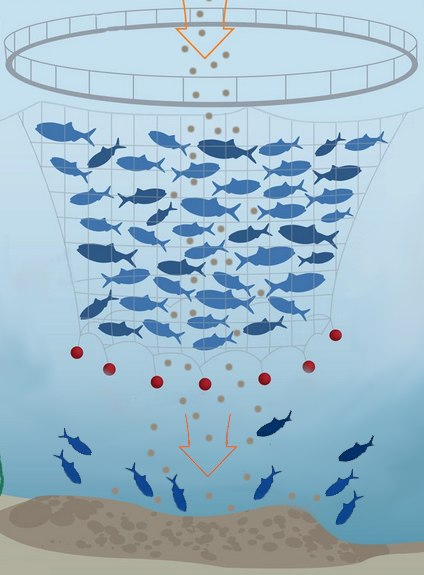
\includegraphics[scale=0.7]{figures/merder-fisk}
\caption{\small \sl Figuren viser et oppdrettsanlegg \cite{Spruill 2011 s. 12}. Fôret til oppdrettsfisken spises også av villfisk. Oppdrettsbransjen er i konflikt med fiskere som mener oppdrettsnæringen ødelegger fiskeplasser i fjordene med anlegg og reduserer kvaliteten til villfisk som spiser fôrpellets under merdene. \cite{Olsen m.fl. 2018} \label{fig:anlegg}} 
\end{center} 
\end{figure} 

Bacheloroppgaven er gjort i samarbeid med Nofima som en del av Sameksistensprosjektet. \cite{Robertsen 2020}